\documentclass[25pt, a0paper, portrait, margin=0mm, innermargin=15mm, blockverticalspace=15mm, colspace=15mm, subcolspace=8mm]{tikzposter}

% useful packages
\usepackage{adjustbox}
\usepackage{multicol}
\usepackage[colalign]{myposter}

% define where to find graphics
\graphicspath{ {images/} {../design_document/images/} }

\usetheme{Wave}
\usebackgroundstyle{Rays}
\usenotestyle{Sticky}
\useblockstyle{TornOut}

% define size of poster
\geometry{paperwidth=36in,paperheight=48in}

% define minnetronix logo
%\newcommand\insertlogoi[2][]{\def\@insertlogoi{\includegraphics[#1]{#2}}}
%\newcommand\insertlogoii[2][]{\def\@insertlogoii{\includegraphics[#1]{#2}}}
%\newlength\LogoSep
%\setlength\LogoSep{0pt}

%\insertlogoi[width=5cm]{example-image-a}
%\insertlogoii[width=5cm]{example-image-b}

\author{Timothy Dee, Justin Long, \& Brandon McDonnell}

\title{Remotely Connected Electric Field Generator \\
for Particle Separation in a Fluid}

%\title{title}
%\author{author}
\institute{Team May1612}

\renewcommand{\baselinestretch}{.8}
\begin{document}

\maketitle

\begin{columns}
\column{.5}

\block{Minnetronix}
{
\begin{tikzfigure}

\includegraphics[width=0.15\textwidth]{images/minnetronix_logo.png}
\end{tikzfigure} 

% say something about Minnetronix
This project is sponsored by
Minnetronix, a health care company based in St. Paul, Minnesota,
founded in 1996.
Minnetronix continues to innovate landscape of health care technology
with an emphasis on device development and commercialization of medical technologies.
This project is apart of this effort.
}

%
% Introduction
%
\block{Problem Statement}
{
\begin{multicols}{2}

This project is part of a larger design to 
exploit the dielectrophoresis phenomenon for
use in medical equipment.
There are many medical applications which
utilize a method of separation.
Centrifuging blood and
testing spinal fluids are two examples of 
such systems.
Current testing equipment is expensive therefore
a cheaper device utilizing DEP would have 
a large competitive advantage if constructed. 

% talk about dielectrophoresis
\textbf{Dielectrophoresis Phenomenon:}
\begin{itemize}
\item separate particles in a fluid.
\item involves applying an electric field to a fluid.
\item field applied over long period of time.
\item particle separation depends on electric field characteristics.
\item adjusting the voltage and frequency used to generate the field 
varies its characteristics.
\end{itemize}

\end{multicols}

%New research has shown that certain particles may be separated from fluids through dielectrophoresis.
%This process involves applying an electric field to a fluid.
%The electric field may then be manipulated in order to attract or repel certain particles.
%The particles the electric field will attract or repel depends on
%characteristics of the electric filed.
%These field characteristics may be controlled
%by varying the voltage and frequency 
%of the electronics driving the field.

% 
%\item Project Basis
%\begin{itemize}
%\item Exploit dielectrophoresis phenomenon for use in medical equipment.
%\item 
%\end{itemize}
%\end{itemize}
}

%\begin{subcolumns}
%\subcolumn{.5}

\subcolumn{.25}

\block{Requirements}
{
\begin{multicols}{2}

% expand upon these requirements
This device will need to be capable of operating in a laboratory environment.
It is also beneficial if this device is portable.
%
Given these constraints, the proposed solution seeks to create a device which is:
\begin{itemize}
\item of small form factor
\item having little cost
\item capable of separating particles in a fluid utilizing DEP
  \begin{itemize}
  \item produces $1$ to $60_{Vpp}$
  \item produces $10_{Khz}$ to $1_{Mhz}$
  \end{itemize}
\end{itemize}

\end{multicols}
}

\block{Solution}
{
\begin{multicols}{2}
%TODO insert picture of Raspberry Pi
%\begin{tikzfigure}
%\includegraphics[width=0.2\textwidth]{images/rpi_real.png}
%\end{tikzfigure}

A number of circuit components connected 
to the the Raspberry Pi GPIO pins.
\begin{itemize}
\item Voltage Control
  \begin{itemize}
  \item Utilizes three Programmable Gain Amplifiers(PGA)
  \item Summing Amplifier to sum the output of PGA's
  \end{itemize}
\item Frequency Control
  \begin{itemize}
  \item Minigen Function Generator
  \item Communicates with Raspberry Pi through SPI
  \end{itemize}
\item Web Interface
  \begin{itemize}
  \item Apache 2 web server hosted on Raspberry Pi
  \item provides user ability to set voltage and frequency output
  \end{itemize}
\end{itemize}

\end{multicols}
}

%
% Testing
%
\block{Testing}
{
%
%TODO split block into two columns
%
\begin{multicols}{2}

%\begin{minipage}[t]{0.1\linewidth}
%text!
%\end{minipage}

%\begin{adjustbox}{valign=t}
%\begin{minipage}[t]{0.1\linewidth}
%text!
%\end{minipage}
%\end{adjustbox}

%TODO include picture
%TODO explain testing environment
A typical testing environment includes:
\begin{itemize}
\item Oscilloscope
\item Raspberry Pi
  \begin{itemize}
  \item Connected for monitor for web interface access
  \item Connected to circuit to control Minigen, PGA's
  \end{itemize}
\item Multiple breadboards
  \begin{itemize}
  \item Minigen Function Generator
  \item PGA's
  \item Summing amplifier
  \end{itemize}
\end{itemize}

%TODO explain testing strategy
Testing this project involved
and iterative process of:
\begin{enumerate}
\item Theorize a design
\item Acquire necessary components
\item Construct design
\item Understand problems
\item Return to step 1
\end{enumerate}
Many times we found that designs would not work
and thus this process began at the beginning.

\end{multicols}
}

%\end{subcolumns}

%
% Design Approach
%
%\note[targetoffsetx=.1\textwidth,targetoffsety=9.5cm,innersep=.4cm,angle=-45,connection]
%{
%Colors denote different functional blocks.
%}

\block{Block Diagram}
{
\begin{multicols}{2}

% insert picture of block diagram
\begin{center}
%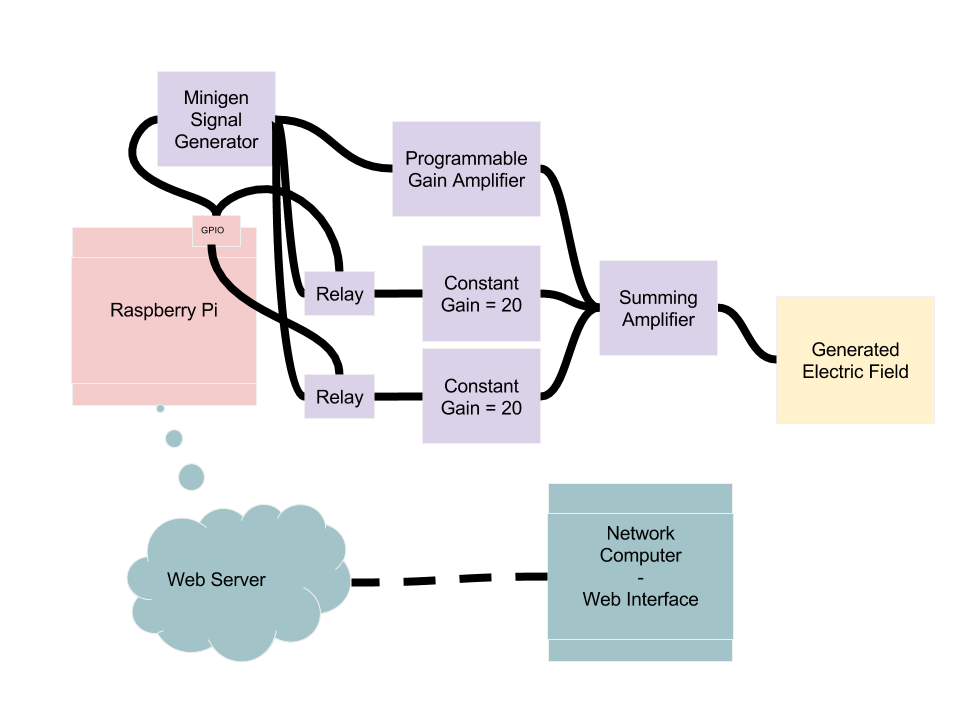
\includegraphics[width=0.35\textwidth,keepaspectratio]{block_diagram.png}
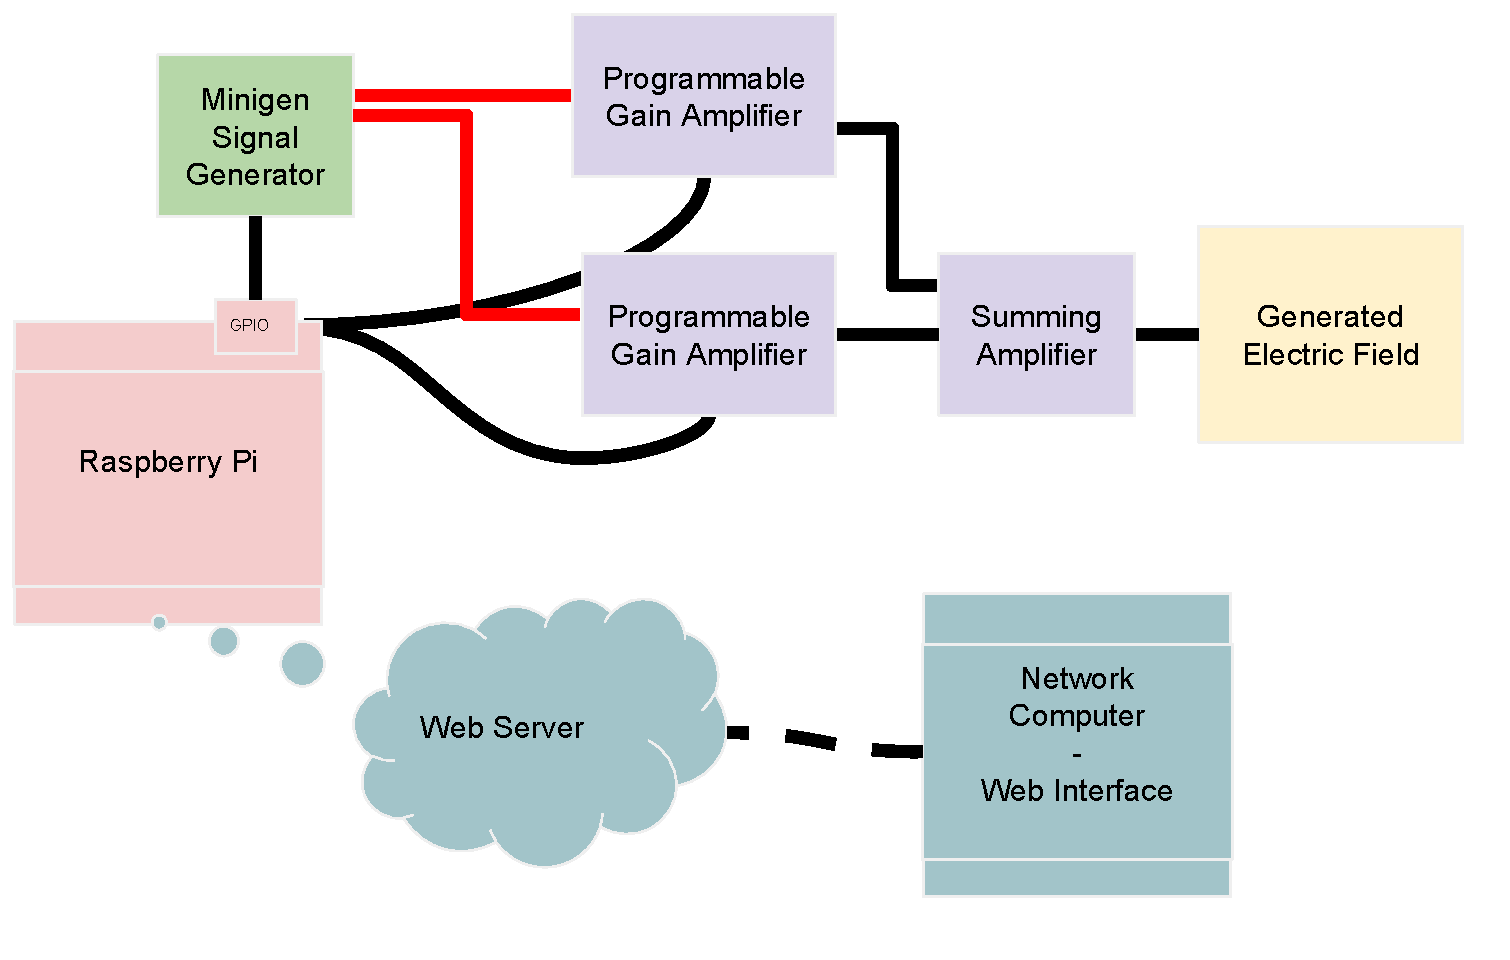
\includegraphics[width=0.2\textwidth,keepaspectratio]{block_diagram.pdf}
\end{center}

%TODO explain each of the functional modules
%TODO explain how each of the functional modules fit together
\textbf{Functional Blocks}
\begin{itemize}
\item Raspberry Pi
  \begin{itemize}
  \item web server
  \item voltage, frequency control scripts
  \end{itemize}
\item MiniGen
\item Amplifier Circuit
%TODO
\end{itemize}

\end{multicols}
}

\column{.5}

%
% Technical Details
%
\block{Raspberry Pi}
{
\begin{multicols}{2}

The Raspberry Pi acts like a bridge between the user and the electronic circuit.
From the perspective of the Pi,
there are two interfaces,
a web server to interact with the human user and
GPIO Pins to interact with the electronic circuit.

% insert Raspberry Pi connection diagram
\begin{center}
\includegraphics[width=0.2\textwidth,keepaspectratio]{rpi_real.png}
\end{center}

%TODO describe what a Raspberry Pi is
\textbf{Raspberry Pi:}
\begin{itemize}
\item Approximately 5.6cm x 8.5cm
\item Running Linux operating system
\item Has 40 General Purpose Input Output (GPIO) pins
%TODO
\end{itemize}

% list important points about web server and GPIO pins
\textbf{Web Server}
\begin{itemize}
\item Implemented using Apache 2 web server.
\item Updates GPIO state using python and bash scripts
\end{itemize}

\textbf{General Purpose Input Output (GPIO) Pins}
\begin{itemize}
\item Connected to PGA's and Minigen
\item SPI communications with Minigen
\item Simple 3-bit interactions with PGA's
\end{itemize}

%The Raspberry Pi will act as the bridge between the user and the circuit.
%The Raspberry Pi will host a web server allowing the user to interact with the system.
%Based on the results of this user interaction, 
%the Raspberry Pi will update the state of the GPIO pins.
%The GPIO pins connect to a circuit causing the output to change based on their state. 

%In addition to hosting the web server the Raspberry pi is used to
%communicate with the 
%Minigen Signal Generator and 
%amplifier circuit.
%This communication is accomplished via 
%the Raspberry Pi's SPI interface and
%GPIO pins respectively.

\end{multicols}
}

\block{Web Interface}
{
\begin{multicols}{2}

%TODO perhaps pictures can be done in note form

\begin{center}
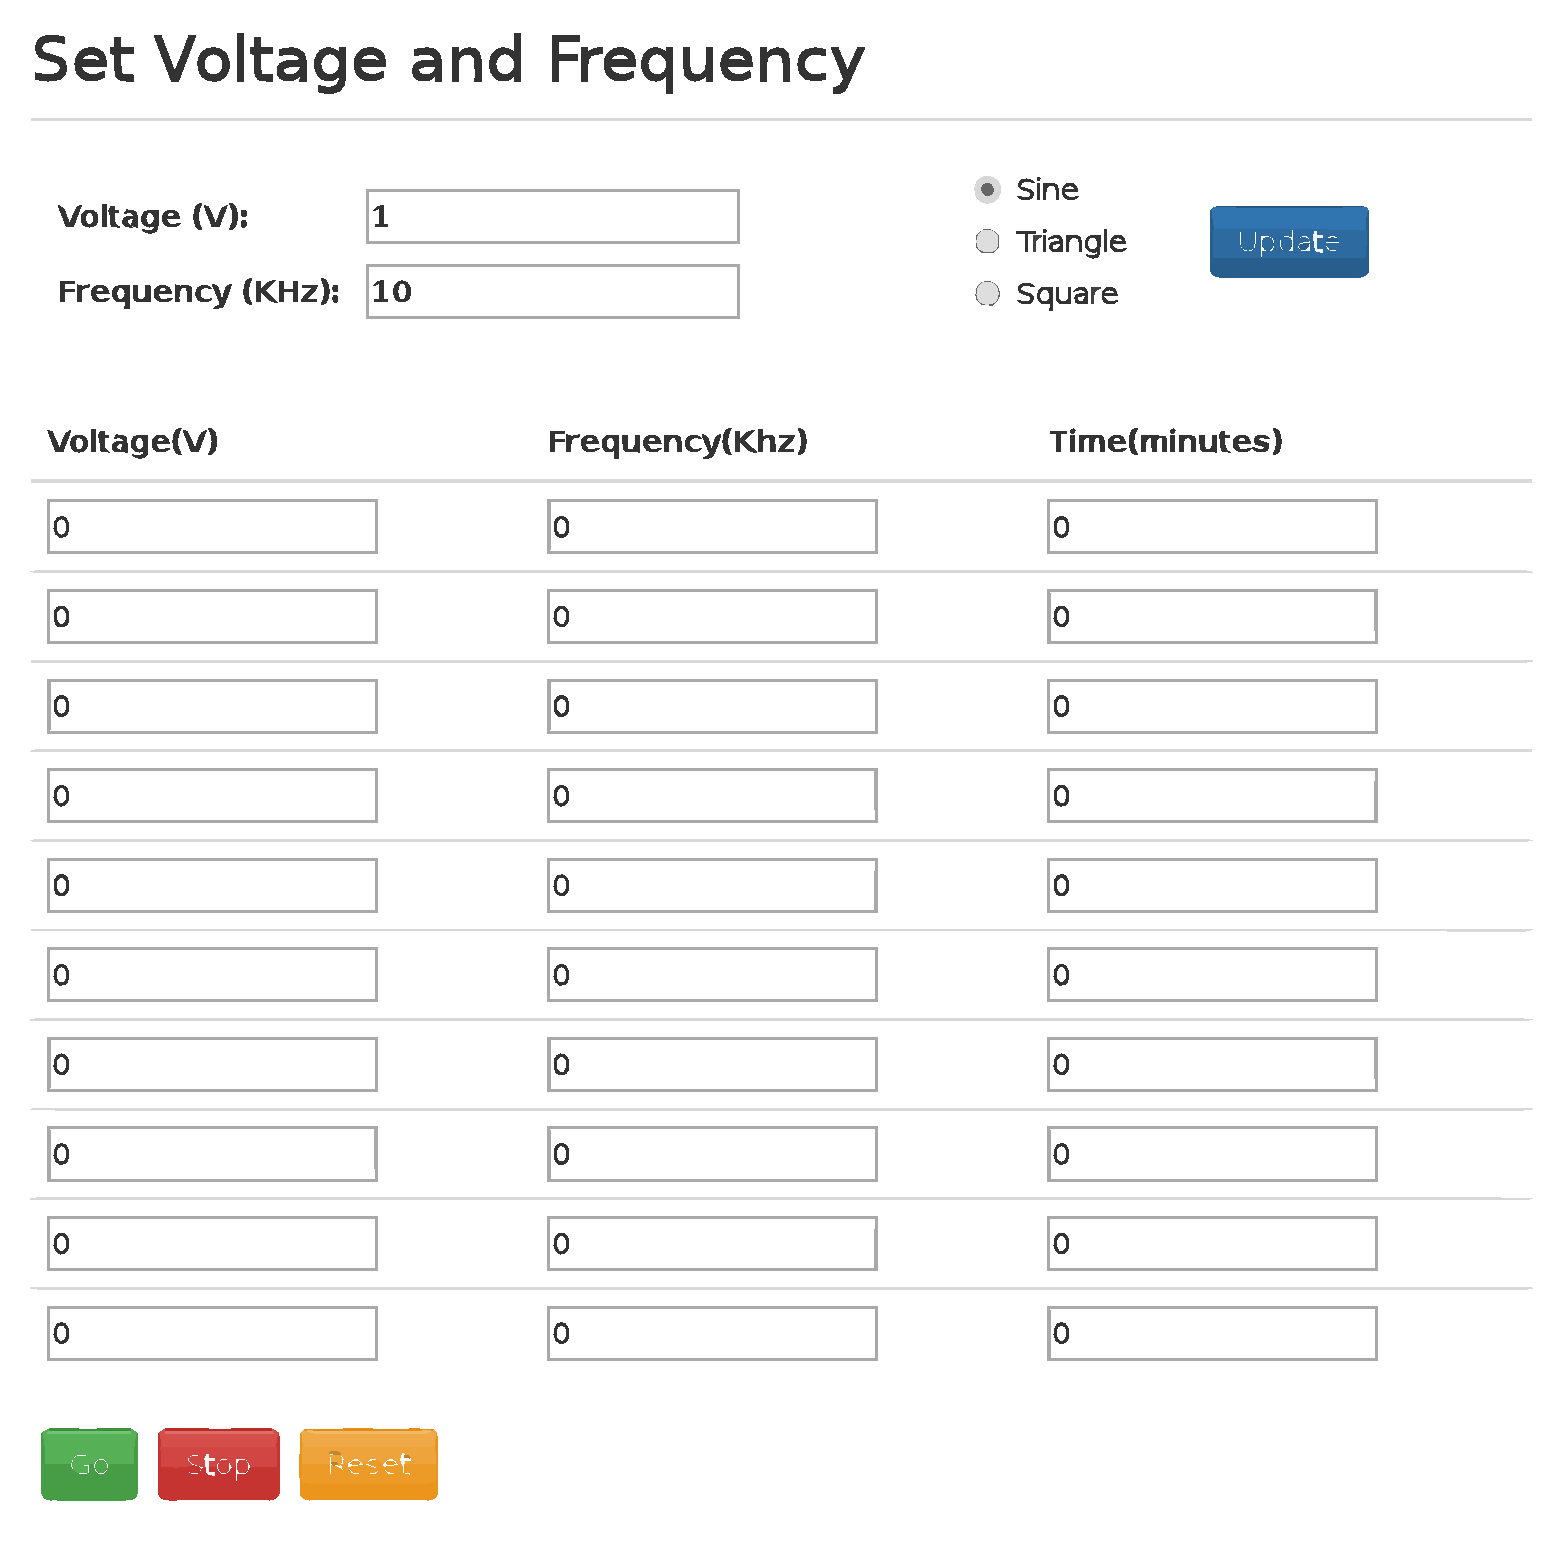
\includegraphics[width=0.2\textwidth,keepaspectratio]{web_interface.pdf}
\end{center}

%TODO insert picture of 
%TODO describe role in design 
\textbf{Interface Specifications}
\begin{itemize}
\item Displayed using Apache 2 web server 
\item Provides functionalities
\begin{itemize}
\item set voltage
\item set frequency
\item adjust signal type, sine, square, and triangle
\item table allows voltage, frequency for time duration in series
\end{itemize}
\item Implemented using cgi-scripts.
\end{itemize}
%TODO

%The web interface is hosted on the Raspberry Pi using an Apache web server.
%This web server displays an interface which allows the user to
%set a voltage and frequency output by the system. 
%The interface is simple and interactive,
%implemented using cgi-scripts on the Apache web server.

%Our implementation provides several functionalities.
%Among these are
%the ability to set:
%voltage and frequency,
%sine or triangle or square waveforms,
%and the ability to set a voltage and frequency for an amount of time.
%The table displayed
%in the figure below
%provides the ability to set voltage and frequency for the number
%of minutes specified.
%The "Go" button will cause the first
%voltage and frequency to be set for the corresponding amount of time.
%After the time has expired,
%the next voltage and frequency will be set for the corresponding amount of time.
%This process continues until the table entries are completed or
%the user presses the "Stop" button.

\end{multicols}
}

\block{Minigen}
{
\begin{multicols}{2}
%The voltage output by the Minigen is not variable.
%Given that the design specification requires a variable voltage,
%the voltage needs to be adjusted separately.
%Accordingly, the output of the Minigen 
%is supplied to the input of the amplifier circuit.

%TODO insert picture of 
%\begin{multicols}{2}
\begin{center}
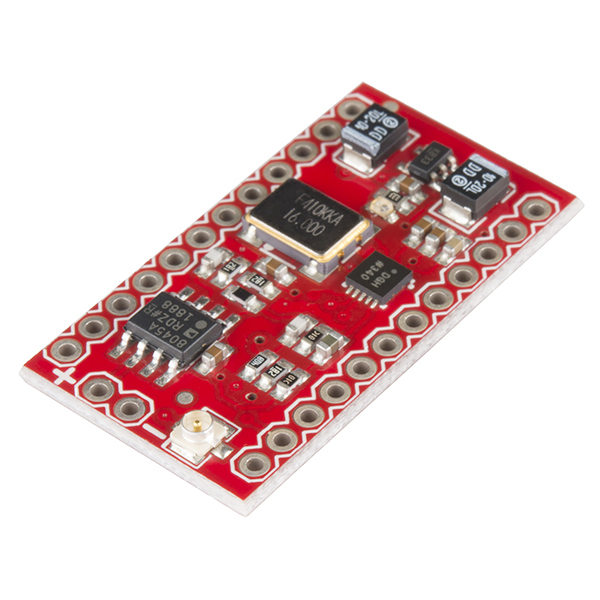
\includegraphics[width=0.1\textwidth,keepaspectratio]{minigen_real.png}
\end{center}
%stuff
%\end{multicols}

%TODO describe role in design 
\textbf{Specifications}
\begin{itemize}
\item Variable frequency integrated circuit device
\item Interconnections
  \begin{itemize}
  \item Frequency set over SPI by Raspberry Pi
  \item Output supplies PGA's input
  \end{itemize}
\item Output waveform
  \begin{itemize}
  \item can output sine, square, triangle waveforms
  \item amplitude $1V_{pp}$
  \item from $-0.5V$ to $0.5V$ 
  \end{itemize}
\item Register Interactions
  \begin{itemize}
  \item 2 frequency registers
    %\begin{itemize}
    %\item 28-bit registers
    %\item one active register controlling output
    %\item can write inactive register
    %\item writing then switching avoids noise in writing register
    %\end{itemize}
  \item 1 control register 
    \begin{itemize}
%    \item modify frequency writes, course or fine
    \item set output waveform
    \end{itemize}
  \end{itemize}
\item Small form factor
\end{itemize}

%The Minigen Function Generator device controls the frequency output by the circuit.
%Varying the frequency is accomplished 
%by writing to registers present on the Minigen.
%This communication is completed over SPI between
%the Raspberry Pi and the Minigen.
%The frequency produced is a function of
%the values contained in the Minigen's frequency registers.

%The Minigen outputs a waveform 
%from -0.5V to 0.5V. 
%This waveform may be a triangle, square, or sine wave.

%The Minigen is controlled by setting five registers,
%two registers for frequency, 
%two for phase shift and 
%one as a control. 
%There exists no need for phase shifting
%to meet the design requirements, 
%however the frequency and control registers
%are needed. 
%By having two frequency registers,
%data can be sent to one register while it is not in use,
%followed by a write to the control register to use this register.
%This allows for a nicer gradient, 
%because the frequency will not change until the entire frequency register is written. 
%The control register also allows for changing between sine, square and triangle waveforms.
%In the event that the frequency needs to be finely adjusted,
%this system utilizes the functionality of the control register
%to modify the way in which writes to the frequency registers are received.
%The way writes are received by the frequency registers 
%can be varied between two modes.
%In one mode,
%two consecutive 14-bit writes to a frequency register are used.
%In the other mode,
%one write to the lower 14-bits of the 28-bit frequency register is used.
%This functionality affords the ability to accurately dial in small changes to the register values quickly.

%Until this point,
%several functional benefits of the Minigen Signal Generator have been discussed.
%An additional benefit which 
%increases the practicality of this solution is the Minigen's small form factor.
%The small chip size 
%allows the Minigen to fit easily into a small case 
%with the Raspberry Pi.
%This is consistent with the system's requisite small footprint.

\end{multicols}
}

\block{Amplifier}
{
\begin{multicols}{2}
%TODO insert picture of amplifier diagram
\begin{center}
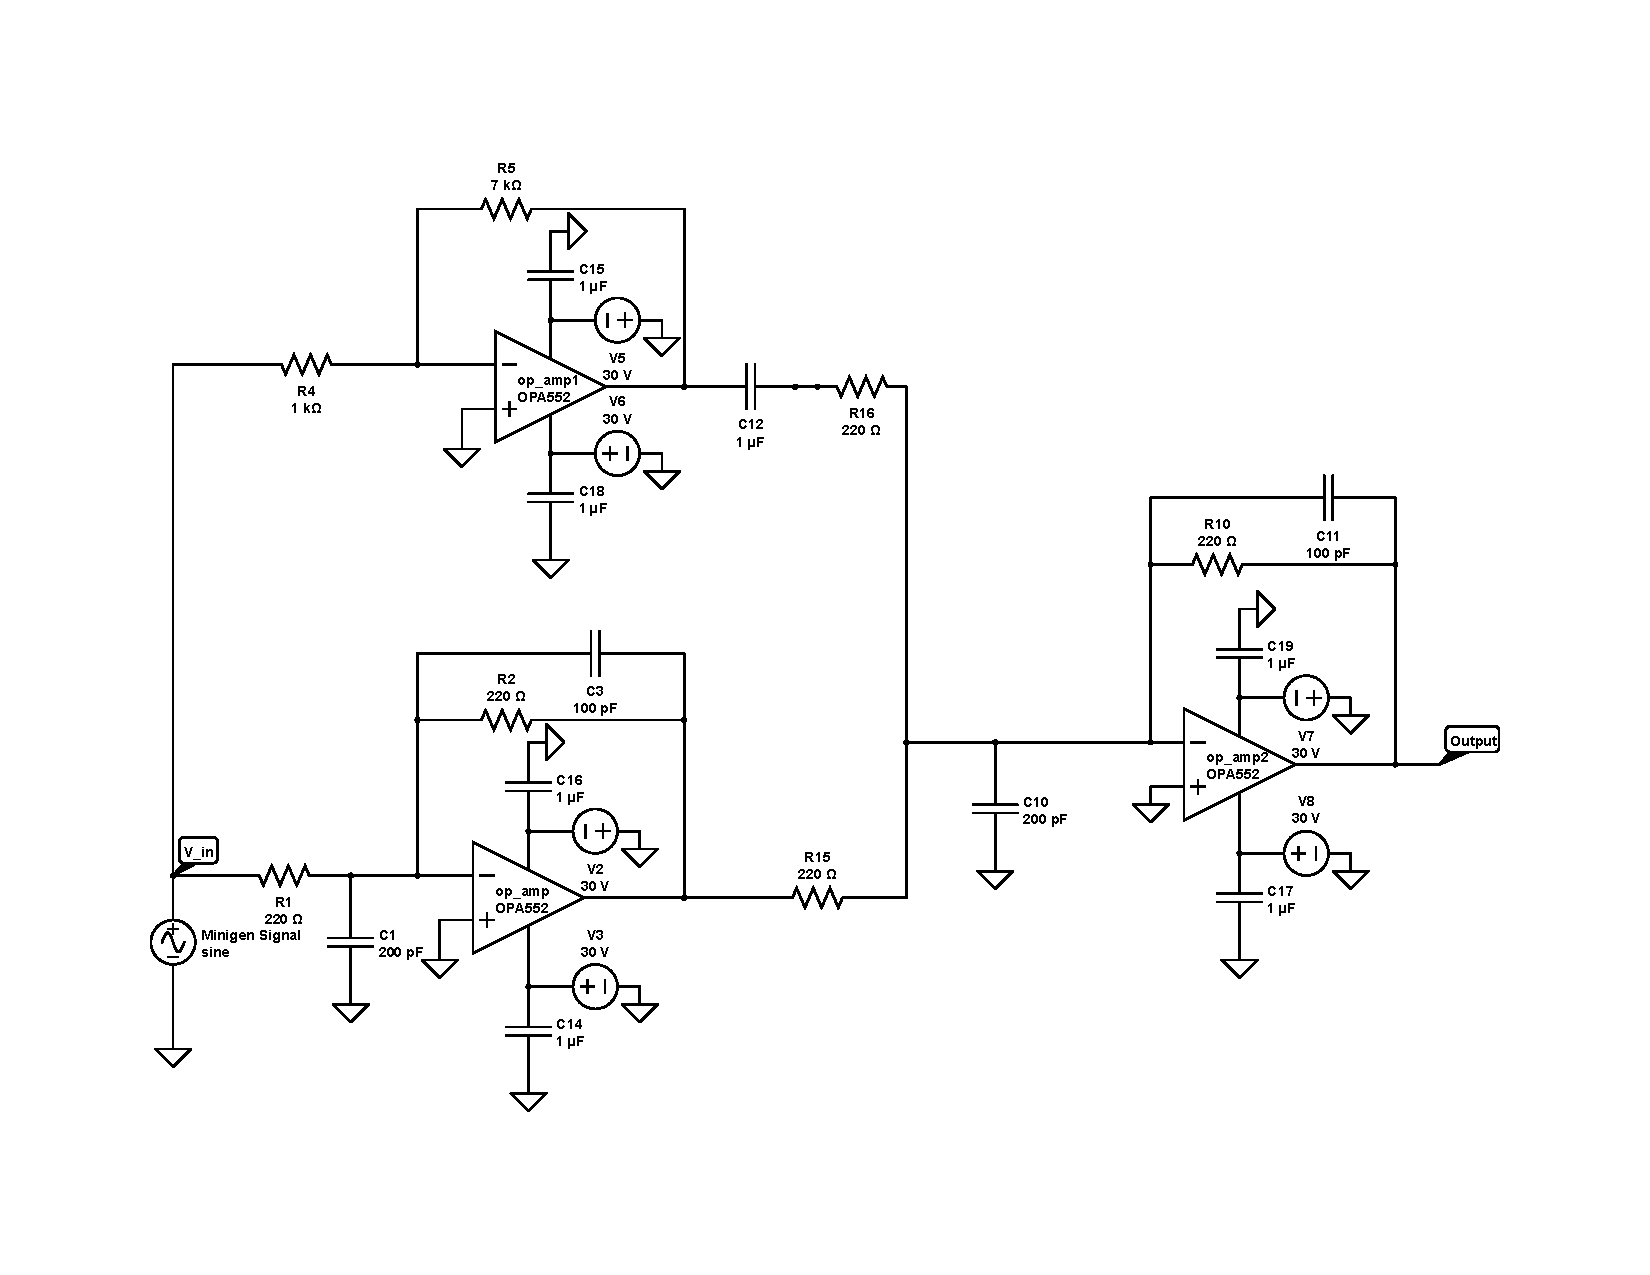
\includegraphics[width=0.23\textwidth,keepaspectratio]{circuit_diagram.pdf}
\end{center}

\newpage

%TODO describe role in design 
\textbf{Components}
\begin{itemize}
\item Programmable Gain Amplifiers (PGA's)
\begin{itemize}
\item Take input from output of Minigen
\item Input to Amplification Stage
\end{itemize}

\item Amplification Stages
\begin{itemize}
\item 3 stages
\item each additional stage gives\\ $\frac{previous\_stage\_step\_size}{7}$
\item takes output of PGA as input
\item outputs to summing amplifier
\end{itemize}

\item Summing Amplifier
\begin{itemize}
\item takes input from amplification stages
\item output is overall circuit output
\item gain of $1V_{pp}$
\end{itemize}

\end{itemize}
%TODO

%As mentioned in the previous section,
%the output of the Minigen Function Generator
%is applied to the amplifier circuit as input.
%The amplifier also receives input from 
%the GPIO pins of the Raspberry Pi.
%These GPIO pins act as switches which help to control the output voltage.
%Based on these inputs 
%the amplifier circuit manages the overall 
%voltage and frequency output.

%The project requirements state that the system must 
%generate signals which range from $1V_{pp}$ to $60V_{pp}$. 
%To accomplish this,
%various circuit components were used to accomplish the amplification.
%The overall scheme is to split the output voltages into
%three different ranges.
%One component is used to adjust the voltage within each of the ranges while
%other comp are used to change the range the voltage adjuster is acting within.

\end{multicols}
}

\end{columns}
\end{document}